While the main strategy for signal extraction uses Multivariate algorithms, but
we have optimised a basic selection using standard discriminating variables
that can be used for increasing the signal-over-background ratio for various studies.

% - Description of the background
The background is made up of two distinctly behaving components: combinatorial background
and \lq B-like\rq\, background. The combinatorial background arises from the random
combination of unrelated tracks in the detector. The \lq B-like\rq\, decays arise from
similar decays involving B mesons, in which one or more of the final state particles
are misidentified and so lead to the event being reconstructed as a $B_{d}^{0} \xrightarrow{} K^{*}e^{+}e^{-}$ event.
One problem, however, is that the background events consist of an overwhelming combinatorial component,
this component of the background is more trivially modelled than \lq B-like\rq\,background,
than the and so obscures our ability to deal with this type of background event.

% - Idea behind the CRS
A Continuum Reduction Selection (CRS), which uses lifetime-related variables that can clean up
the overwhelming combinatorial background, was then implemented. This allows us to study and
produce the data-MC comparison plots. Furthermore, it may allow us to focus on the
\lq B-like\rq\,background characterisation and modelling.

% - The variables used in the CRS and their definitions
In order for a variable to discriminate between signal-like and combinatorial decays,
we want it to exploit the inherent difference between the decays, that signal-like decays
correspond to real particles (whether misreconstructed or not). As such, we expect
signal-like events to have a longer lifetime and larger values for other variables
proportional to the lifetime. The variables considered in the CRS are:
$\tau_{B}$ -- the lifetime of the B, $L_{\textrm{xy}}$ -- the displacement of the $J/\psi$
vertex from the PV, projected onto the flight direction of the $J/\psi$
in the transverse plane, and $\cos \theta$ -- the cosine of the angle between the vector
joining the PV and SV, and the direction of flight of the B. The significance values
(i.e. the variable divided by its error) of these variables are also considered in the
optimisation of the CRS.

% - CRS optimisration incl. fits
To optimise our cuts, in order to most efficiently cut away combinatorial background
without also removing the signal, we must define some efficiency. In this optimisation,
the Punzi significance \cite{Punzi} was used, which has advantages over the traditional
method of calculating the significance $Z = S/\sqrt{S+B}$, which is used for comparing
an existing signal with the overall statistical uncertainty in the Poissonian event count.
The Punzi significance is used when we are uncertain of the cross-section we should expect,
which will inevitably be factored in when we want to give an estimate for the signal yield.
For the $R(K^{*})$, the large uncertainties on the $b\Bar{b}$ cross-section make the use
of the Punzi significance necessary. Instead of the signal yield, we optimise using the
efficiency of the cut on signal. This efficiency is calculated from the percentage of
the MC events passing a given cut. Explicitly, the Punzi significance is calculated as
\begin{equation}
    Z_{\textrm{Punzi}} = \frac{\epsilon(t)}{a/2 + \sqrt{B(t)}},
    \label{eq:punzicalc}
\end{equation}
where $\epsilon(t)$ is the signal efficiency, $a$ the number of sigma deviations
(corresponding to one-sided Gaussian test, at some significance $\alpha$),
and $B(t)$ the number of background events passing the cut, at threshold $t$.
This also allows us to optimise the cuts without knowing the form of the signal
in the data \textit{a priori}, and to optimise our cuts on the blinded signal
significance in the low-$q^{2}$ region.

% - CRS applied plots
\begin{figure}[]
    \centering
    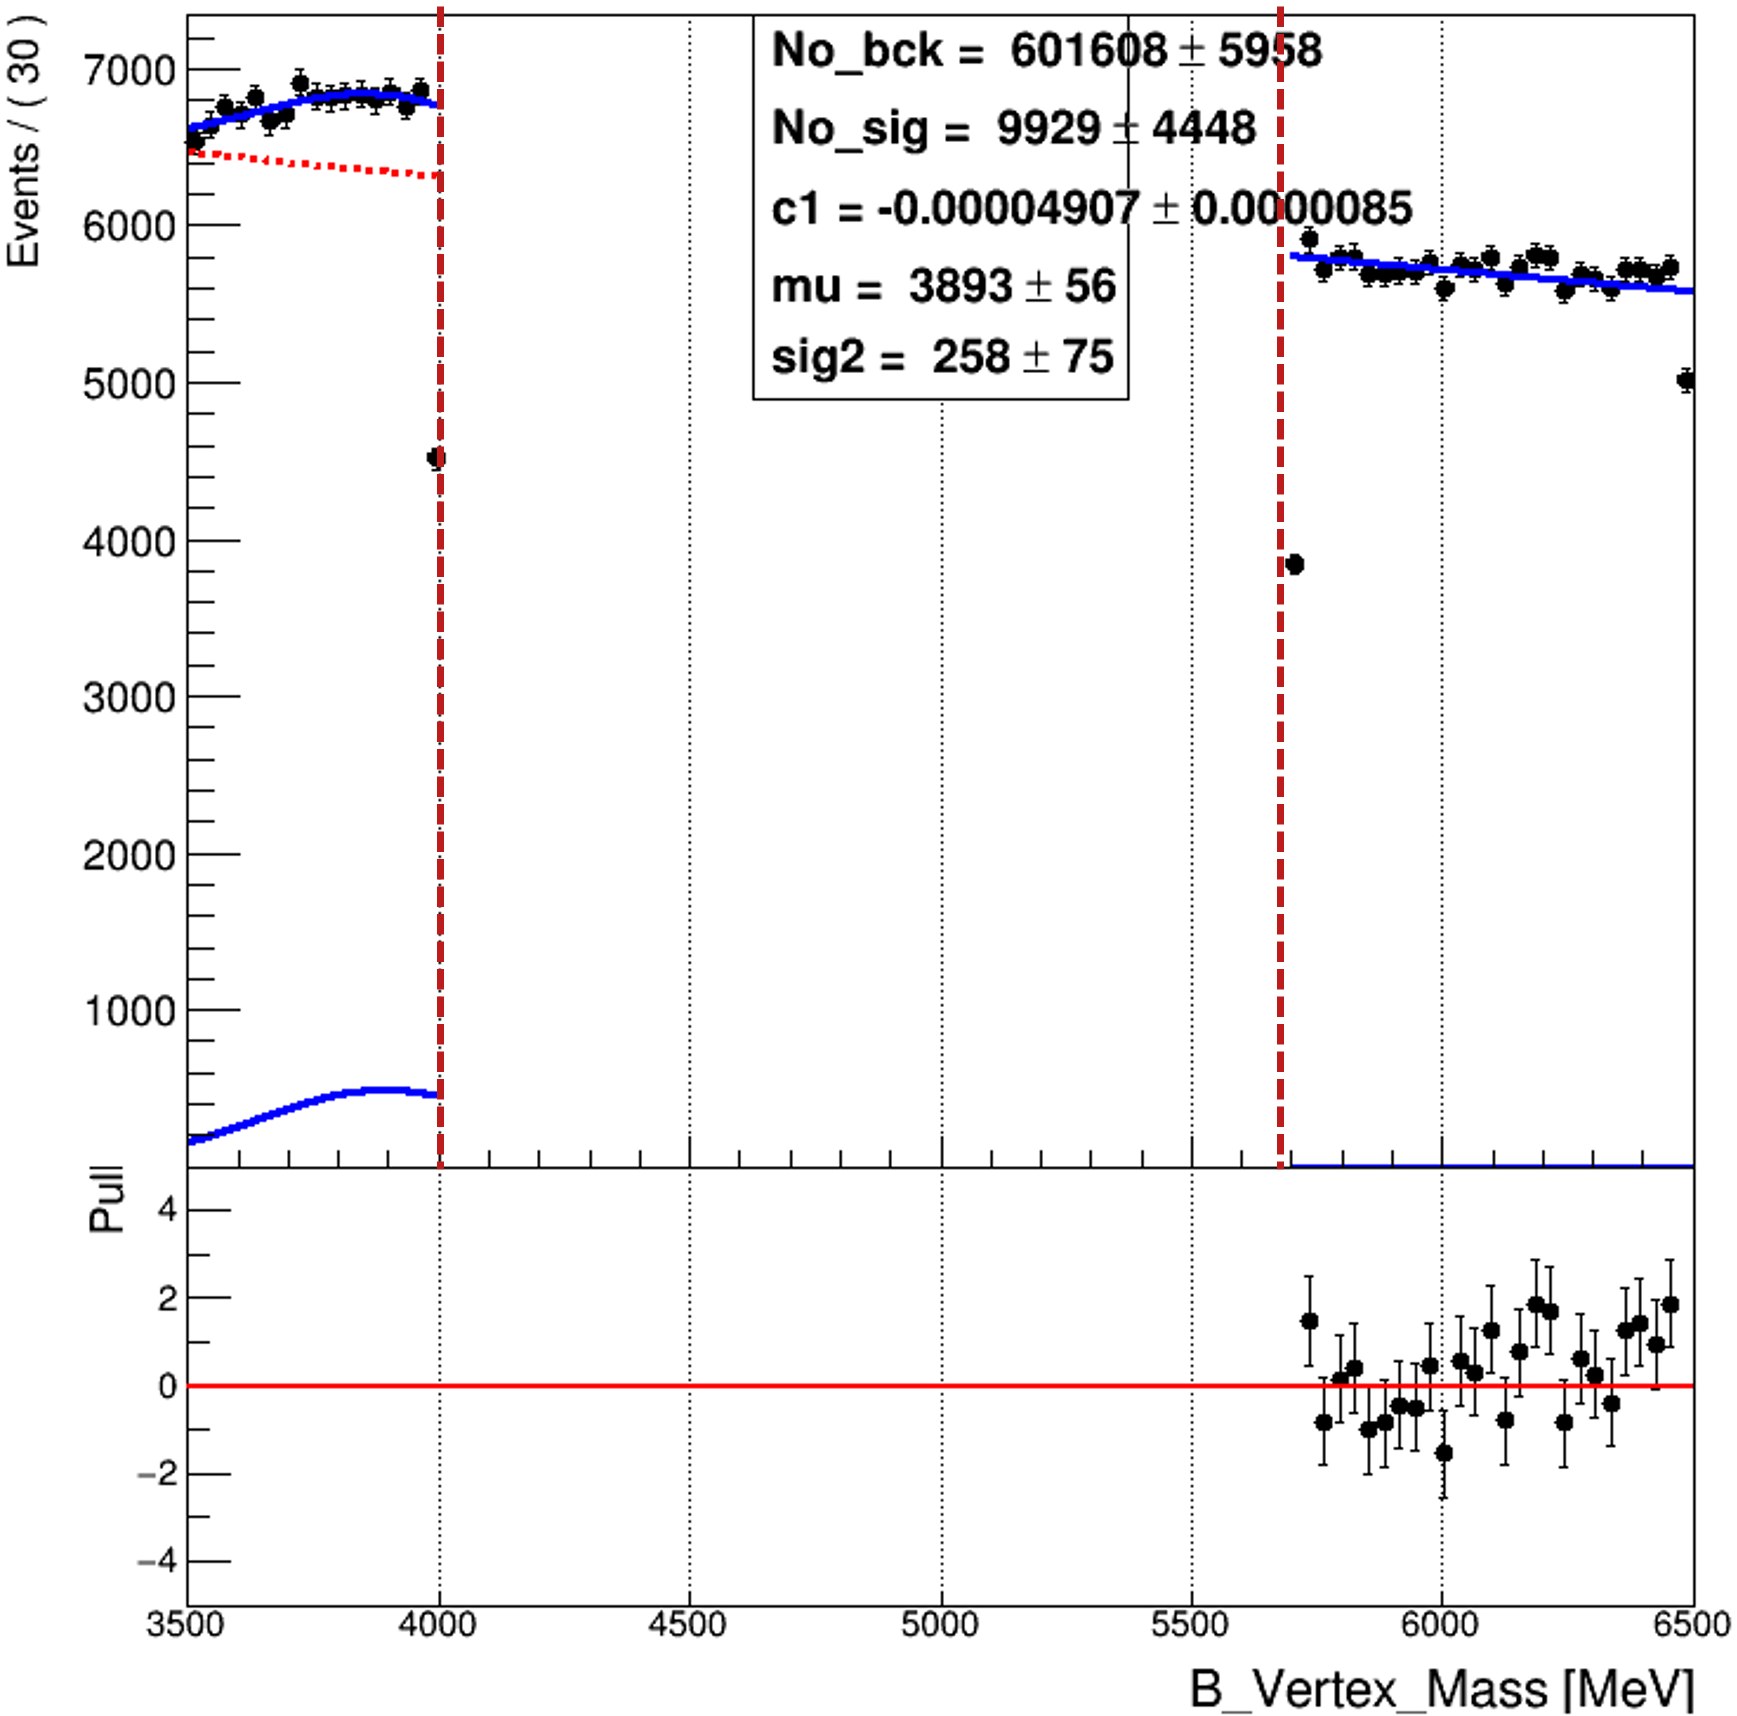
\includegraphics[width=0.5\textwidth]{figures/SidebandFit_CRSoptimisation.png}
    \caption{A blinded extended-likelihood fit to the invariant B mass in the low-$q^{2}$ signal region.
    Here the background shape is modelled by an exponential (combinatorial component) and a
    wide Gaussian (\lq B-like' background component). Below the pulls for the fit are also
    shown for the high-mass sideband.}
    \label{fig:SBFitCRS}
\end{figure}

To perform the 2D optimisation of the CRS, two CRS variables needed to be chosen.
These variables must have both good discriminating power between combinatorial
and \lq signal-like' decays and also exploit the information about the data.
To choose the first of the two variables, a significance scan was performed
on each of the CRS variables and the Punzi significance calculated at each
point in the scan (corresponding to varying the cut of each CRS variable).
In calculating the Punzi significance, the $\epsilon(t)$ was calculated as
the fraction of signal MC passing the cut, the value of $a$ was taken as 2,
and the background was calculated from a fit to the blinded low-$q^{2}$
sideband data. Here, assuming the sideband is a good approximation to the background,
we can calculate the number of background events $B(t)$ passing the cut
by rescaling our signal yield in the sidebands by the fraction of the blinded fit yield
in the signal region and sideband region. The blinded signal region of the low-$q^{2}$
data is defined as $m_{B} \in [4, 5.7]$\,GeV, whereas the sideband is defined
as the region $m_{B} \in [3.5, 4] \cup [5.7, 6.5]$\,GeV. Fig. \ref{fig:SBFitCRS}
shows the blinded fit to the low-$q^{2}$ invariant B mass distribution.
The signal-to-sideband ratio of the blinded fit yield is seen to be 0.567:0.433,
giving a normalisation factor of 1.31. The denominator in Eq.~\ref{eq:punzicalc}
can then be expressed as $1 + \sqrt{1.31B_{\textrm{SB}}(t)}$.
\begin{figure}[]
    \centering
    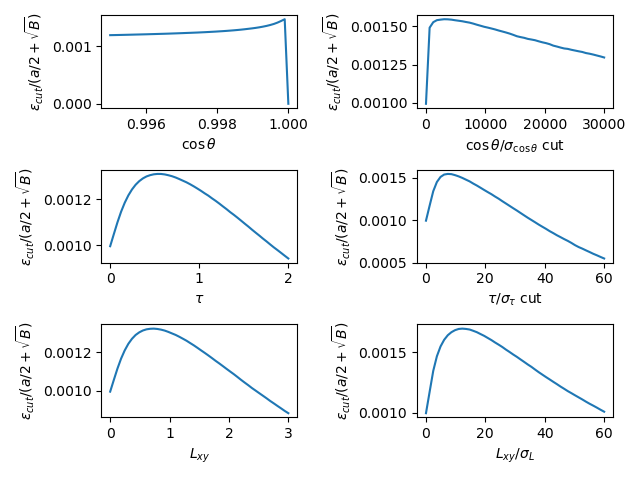
\includegraphics[width = 0.5\textwidth]{figures/PunziScan.png}
    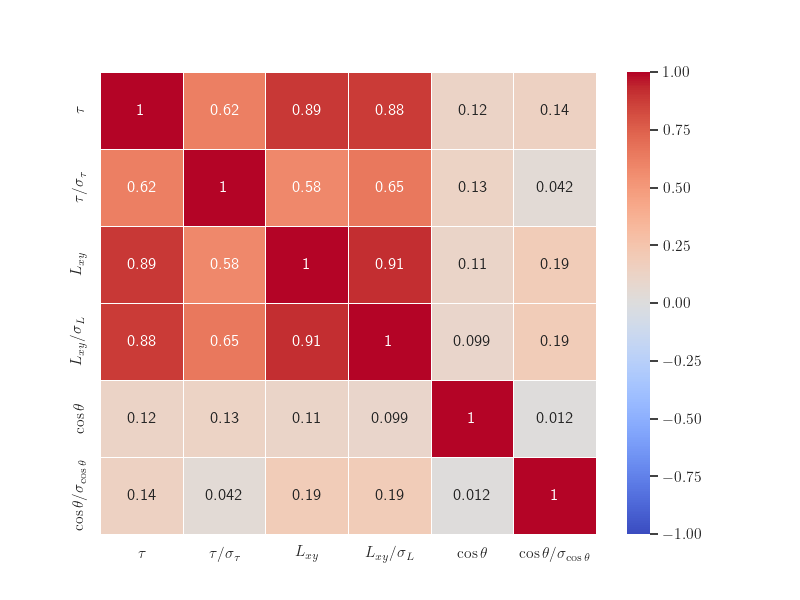
\includegraphics[width = 0.4\textwidth]{figures/CRSVarCorrs.png}
    \caption{Punzi significance scans for each of the 6 variables in the CRS optimisation,
    here the $L_{\textrm{xy}}$ significance value has the peak Punzi significance (left).
    The linear correlation coefficients between the various CRS variables (right).}
    \label{fig:PunziScans}
\end{figure}

For each of the Punzi significance scans, shown in Fig. \ref{fig:PunziScans}, the peak
significance was taken. These were then compared and the CRS variable with the highest
peak Punzi significance was chosen as the first variable for optimisation in the CRS.
This is seen to be the $L_{\textrm{xy}}$ significance. It is worth noting that
the Punzi significance does not correspond to a physically meaningful significance,
nor a sensitivity, instead, its maximum corresponds to a maximum sensitivity measurement,
i.e. by maximising the Punzi significance of our CRS scan we maximise our sensitivity
to the signal.

\begin{figure}
    \centering
    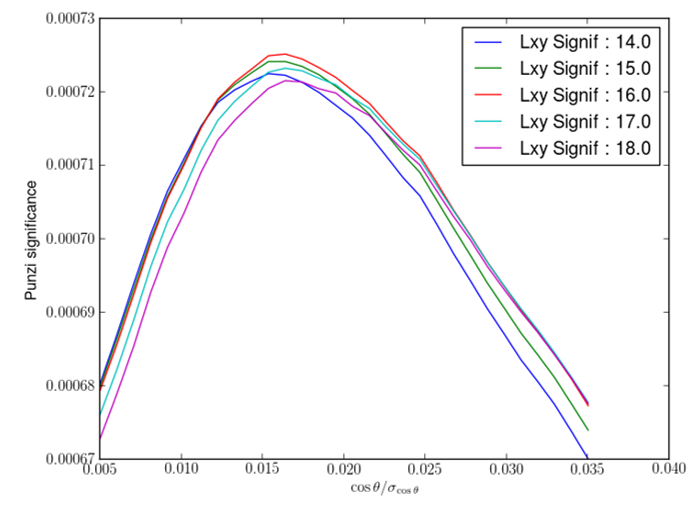
\includegraphics[width = 0.5\textwidth]{figures/2DPunziOpt.png}
    \caption{2D optimisation performed by scanning the Punzi significance of
    $\cos \theta$ significance cuts, for a given cut on the $L_{\textrm{xy}}$ significance.}
    \label{fig:2DCRSOpt}
\end{figure}

For choosing the second variable to be optimised, and with the idea of choosing the remaining
variable which would exploit the most information about the data, the correlations between
the CRS variables were calculated. These are shown in Fig \ref{fig:PunziScans}.
Having chosen the $L_{\textrm{xy}}$ significance as the first variable in the 2D CRS optimisation,
the second variable is the one with the smallest correlation coefficient with $L_{\textrm{xy}}$,
which is seen to be the $\cos \theta$ significance.
Finally, the 2D optimisation of the cuts in $(L_{\textrm{xy}}/\sigma_{L}, \cos \theta/\sigma_{\cos \theta})$
was done by performing a grid search maximisation of the Punzi significance for pairs of cuts.
Fig~\ref{fig:2DCRSOpt} shows the Punzi significance scan for a few slices of the grid search.
Optimum cuts on $(L_{\textrm{xy}}/\sigma_{L}, \cos \theta/\sigma_{\cos \theta})$ were found
to be $L_{\textrm{xy}}/\sigma_{L} >  15.8, \cos \theta/\sigma_{\cos \theta} > 0.016$.
\begin{figure}
    \centering
    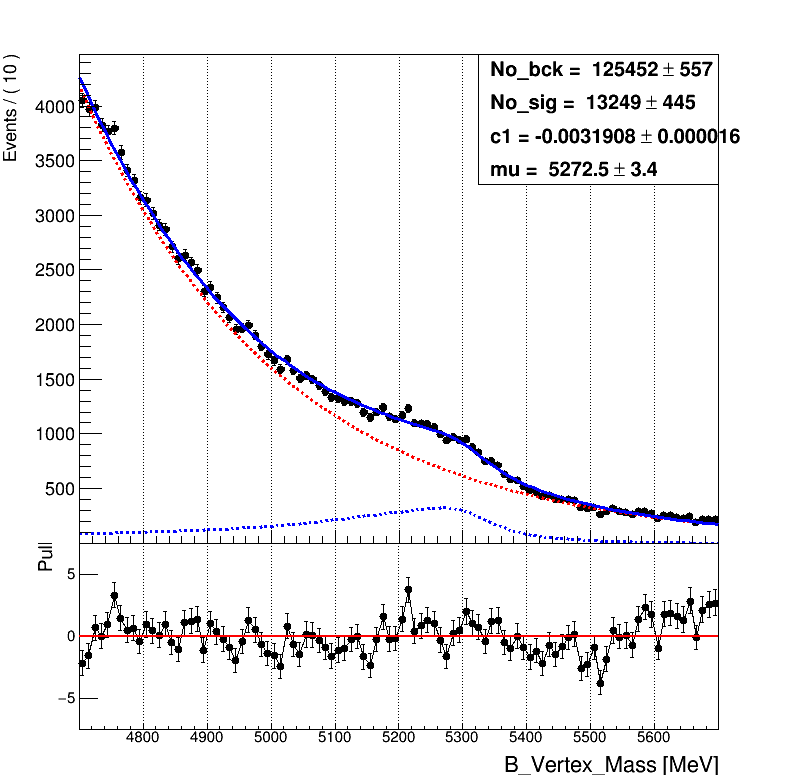
\includegraphics[width = 0.4\textwidth]{figures/B_masses_cutflow_JPsi_highq2_datafit.png}
    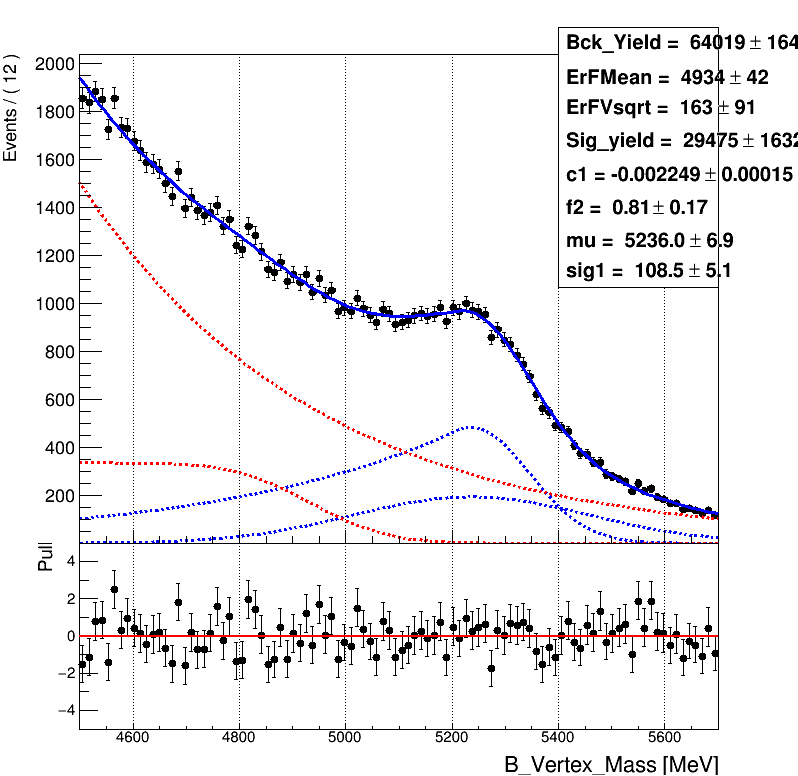
\includegraphics[width = 0.4\textwidth]{figures/BmassFit_Jpsi_Data_Highq2_CRS_extended_Bkgpdf_erfc_cores_free.png}
    \caption{(Left) Extended likelihood fits to the invariant B mass, with only the preselection applied,
    here signal is shown in blue and background in red. The fit results are also shown.
    (Right) Extended likelihood fits to the invariant B mass, with the preselection and
    additional CRS applied, here signal is shown in blue and background in red.
    The fit results are also shown. }
    \label{fig:CRSvsCutflowFits}
\end{figure}

The optimised CRS was then applied to the low-$q^{2}$ sideband data and also high-$q^{2}$ data
to assess the effect of the optimised selection on the reduction of combinatorial background.
For the high-$q^{2}$, this is particularly insightful as to the efficacy of the CRS,
as we see the emergence of the $J/\psi$ mass peak from the overwhelming background.
Fig.~\ref{fig:CRSvsCutflowFits} shows extended likelihood fits to the invariant B mass,
with and without the CRS applied. As can be seen, the CRS gives us a much better handle
on the functional form of the signal shape and allows us to safely factor
in the contribution of the \lq B-like' backgrounds in the background.
